\documentclass[twoside]{book}

% Packages required by doxygen
\usepackage{fixltx2e}
\usepackage{calc}
\usepackage{doxygen}
\usepackage[export]{adjustbox} % also loads graphicx
\usepackage{graphicx}
\usepackage[utf8]{inputenc}
\usepackage{makeidx}
\usepackage{multicol}
\usepackage{multirow}
\PassOptionsToPackage{warn}{textcomp}
\usepackage{textcomp}
\usepackage[nointegrals]{wasysym}
\usepackage[table]{xcolor}

% Font selection
\usepackage[T1]{fontenc}
\usepackage[scaled=.90]{helvet}
\usepackage{courier}
\usepackage{amssymb}
\usepackage{sectsty}
\renewcommand{\familydefault}{\sfdefault}
\allsectionsfont{%
  \fontseries{bc}\selectfont%
  \color{darkgray}%
}
\renewcommand{\DoxyLabelFont}{%
  \fontseries{bc}\selectfont%
  \color{darkgray}%
}
\newcommand{\+}{\discretionary{\mbox{\scriptsize$\hookleftarrow$}}{}{}}

% Page & text layout
\usepackage{geometry}
\geometry{%
  a4paper,%
  top=2.5cm,%
  bottom=2.5cm,%
  left=2.5cm,%
  right=2.5cm%
}
\tolerance=750
\hfuzz=15pt
\hbadness=750
\setlength{\emergencystretch}{15pt}
\setlength{\parindent}{0cm}
\setlength{\parskip}{0.2cm}
\makeatletter
\renewcommand{\paragraph}{%
  \@startsection{paragraph}{4}{0ex}{-1.0ex}{1.0ex}{%
    \normalfont\normalsize\bfseries\SS@parafont%
  }%
}
\renewcommand{\subparagraph}{%
  \@startsection{subparagraph}{5}{0ex}{-1.0ex}{1.0ex}{%
    \normalfont\normalsize\bfseries\SS@subparafont%
  }%
}
\makeatother

% Headers & footers
\usepackage{fancyhdr}
\pagestyle{fancyplain}
\fancyhead[LE]{\fancyplain{}{\bfseries\thepage}}
\fancyhead[CE]{\fancyplain{}{}}
\fancyhead[RE]{\fancyplain{}{\bfseries\leftmark}}
\fancyhead[LO]{\fancyplain{}{\bfseries\rightmark}}
\fancyhead[CO]{\fancyplain{}{}}
\fancyhead[RO]{\fancyplain{}{\bfseries\thepage}}
\fancyfoot[LE]{\fancyplain{}{}}
\fancyfoot[CE]{\fancyplain{}{}}
\fancyfoot[RE]{\fancyplain{}{\bfseries\scriptsize Generated on Mon Nov 14 2016 02\+:13\+:02 for Equation Computation Project by Doxygen }}
\fancyfoot[LO]{\fancyplain{}{\bfseries\scriptsize Generated on Mon Nov 14 2016 02\+:13\+:02 for Equation Computation Project by Doxygen }}
\fancyfoot[CO]{\fancyplain{}{}}
\fancyfoot[RO]{\fancyplain{}{}}
\renewcommand{\footrulewidth}{0.4pt}
\renewcommand{\chaptermark}[1]{%
  \markboth{#1}{}%
}
\renewcommand{\sectionmark}[1]{%
  \markright{\thesection\ #1}%
}

% Indices & bibliography
\usepackage{natbib}
\usepackage[titles]{tocloft}
\setcounter{tocdepth}{3}
\setcounter{secnumdepth}{5}
\makeindex

% Hyperlinks (required, but should be loaded last)
\usepackage{ifpdf}
\ifpdf
  \usepackage[pdftex,pagebackref=true]{hyperref}
\else
  \usepackage[ps2pdf,pagebackref=true]{hyperref}
\fi
\hypersetup{%
  colorlinks=true,%
  linkcolor=blue,%
  citecolor=blue,%
  unicode%
}

% Custom commands
\newcommand{\clearemptydoublepage}{%
  \newpage{\pagestyle{empty}\cleardoublepage}%
}


%===== C O N T E N T S =====

\begin{document}

% Titlepage & ToC
\hypersetup{pageanchor=false,
             bookmarks=true,
             bookmarksnumbered=true,
             pdfencoding=unicode
            }
\pagenumbering{roman}
\begin{titlepage}
\vspace*{7cm}
\begin{center}%
{\Large Equation Computation Project \\[1ex]\large 1.\+0 }\\
\vspace*{1cm}
{\large Generated by Doxygen 1.8.9.1}\\
\vspace*{0.5cm}
{\small Mon Nov 14 2016 02:13:02}\\
\end{center}
\end{titlepage}
\clearemptydoublepage
\tableofcontents
\clearemptydoublepage
\pagenumbering{arabic}
\hypersetup{pageanchor=true}

%--- Begin generated contents ---
\chapter{Hierarchical Index}
\section{Class Hierarchy}
This inheritance list is sorted roughly, but not completely, alphabetically\+:\begin{DoxyCompactList}
\item exception\begin{DoxyCompactList}
\item \contentsline{section}{argument\+\_\+invalid\+\_\+exception}{\pageref{classargument__invalid__exception}}{}
\item \contentsline{section}{negative\+\_\+number\+\_\+exception}{\pageref{classnegative__number__exception}}{}
\item \contentsline{section}{overflow\+\_\+exception}{\pageref{classoverflow__exception}}{}
\end{DoxyCompactList}
\end{DoxyCompactList}

\chapter{Class Index}
\section{Class List}
Here are the classes, structs, unions and interfaces with brief descriptions\+:\begin{DoxyCompactList}
\item\contentsline{section}{\hyperlink{classargument__invalid__exception}{argument\+\_\+invalid\+\_\+exception} \\*Exception invoked by invalid arguments }{\pageref{classargument__invalid__exception}}{}
\item\contentsline{section}{\hyperlink{classnegative__number__exception}{negative\+\_\+number\+\_\+exception} \\*Exception invoked by negative numbers }{\pageref{classnegative__number__exception}}{}
\item\contentsline{section}{\hyperlink{classoverflow__exception}{overflow\+\_\+exception} \\*Exception invoked by integer overflow }{\pageref{classoverflow__exception}}{}
\end{DoxyCompactList}

\chapter{File Index}
\section{File List}
Here is a list of all documented files with brief descriptions\+:\begin{DoxyCompactList}
\item\contentsline{section}{\hyperlink{code__quality__professional_8cpp}{code\+\_\+quality\+\_\+professional.\+cpp} }{\pageref{code__quality__professional_8cpp}}{}
\end{DoxyCompactList}

\chapter{Class Documentation}
\hypertarget{classargument__invalid__execption}{}\section{argument\+\_\+invalid\+\_\+execption Class Reference}
\label{classargument__invalid__execption}\index{argument\+\_\+invalid\+\_\+execption@{argument\+\_\+invalid\+\_\+execption}}


Exception invoked by invalid arguments.  




Inheritance diagram for argument\+\_\+invalid\+\_\+execption\+:\nopagebreak
\begin{figure}[H]
\begin{center}
\leavevmode
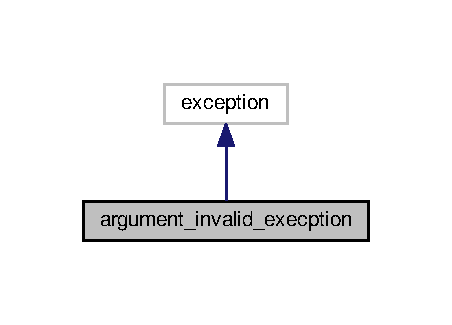
\includegraphics[width=217pt]{classargument__invalid__execption__inherit__graph}
\end{center}
\end{figure}


Collaboration diagram for argument\+\_\+invalid\+\_\+execption\+:\nopagebreak
\begin{figure}[H]
\begin{center}
\leavevmode
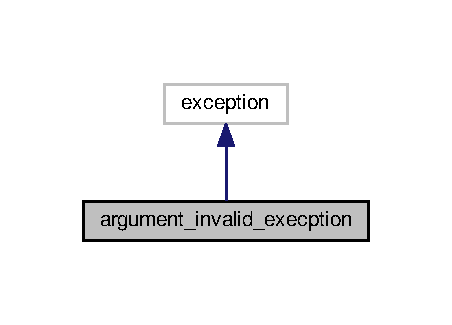
\includegraphics[width=217pt]{classargument__invalid__execption__coll__graph}
\end{center}
\end{figure}
\subsection*{Public Member Functions}
\begin{DoxyCompactItemize}
\item 
virtual const char $\ast$ \hyperlink{classargument__invalid__execption_a195981d8dc3b6f1374c920e63eaf8ba8}{what} () const   throw ()
\begin{DoxyCompactList}\small\item\em Details the problem which invokes the exception. \end{DoxyCompactList}\end{DoxyCompactItemize}
\subsection*{Public Attributes}
\begin{DoxyCompactItemize}
\item 
\hypertarget{classargument__invalid__execption_a294e0bad63968d067685cef34645f856}{}char $\ast$ \hyperlink{classargument__invalid__execption_a294e0bad63968d067685cef34645f856}{argument}\label{classargument__invalid__execption_a294e0bad63968d067685cef34645f856}

\begin{DoxyCompactList}\small\item\em Used to store the argument which is invalid. \end{DoxyCompactList}\end{DoxyCompactItemize}


\subsection{Detailed Description}
Exception invoked by invalid arguments. 

This exception can be used when an input argument is invalid 

\subsection{Member Function Documentation}
\hypertarget{classargument__invalid__execption_a195981d8dc3b6f1374c920e63eaf8ba8}{}\index{argument\+\_\+invalid\+\_\+execption@{argument\+\_\+invalid\+\_\+execption}!what@{what}}
\index{what@{what}!argument\+\_\+invalid\+\_\+execption@{argument\+\_\+invalid\+\_\+execption}}
\subsubsection[{what}]{\setlength{\rightskip}{0pt plus 5cm}virtual const char$\ast$ argument\+\_\+invalid\+\_\+execption\+::what (
\begin{DoxyParamCaption}
{}
\end{DoxyParamCaption}
) const throw  ) \hspace{0.3cm}{\ttfamily [inline]}, {\ttfamily [virtual]}}\label{classargument__invalid__execption_a195981d8dc3b6f1374c920e63eaf8ba8}


Details the problem which invokes the exception. 

\begin{DoxyReturn}{Returns}
A string detailing the exception 
\end{DoxyReturn}


The documentation for this class was generated from the following file\+:\begin{DoxyCompactItemize}
\item 
\hyperlink{code__quality__professional_8cpp}{code\+\_\+quality\+\_\+professional.\+cpp}\end{DoxyCompactItemize}

\hypertarget{classnegative__number__execption}{}\section{negative\+\_\+number\+\_\+execption Class Reference}
\label{classnegative__number__execption}\index{negative\+\_\+number\+\_\+execption@{negative\+\_\+number\+\_\+execption}}


Exception invoked by negative numbers.  




Inheritance diagram for negative\+\_\+number\+\_\+execption\+:\nopagebreak
\begin{figure}[H]
\begin{center}
\leavevmode
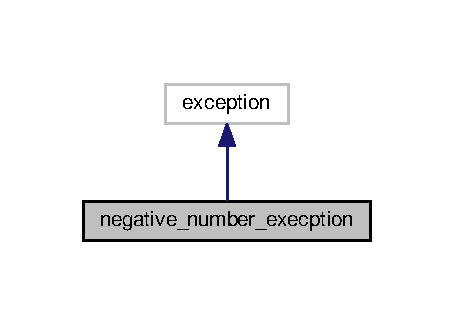
\includegraphics[width=218pt]{classnegative__number__execption__inherit__graph}
\end{center}
\end{figure}


Collaboration diagram for negative\+\_\+number\+\_\+execption\+:\nopagebreak
\begin{figure}[H]
\begin{center}
\leavevmode
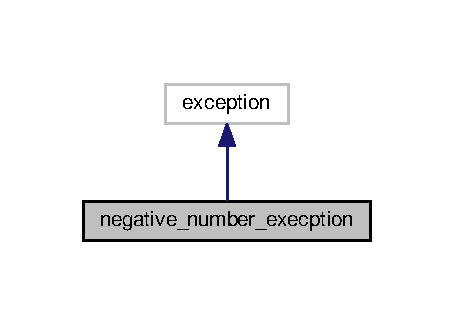
\includegraphics[width=218pt]{classnegative__number__execption__coll__graph}
\end{center}
\end{figure}
\subsection*{Public Member Functions}
\begin{DoxyCompactItemize}
\item 
virtual const char $\ast$ \hyperlink{classnegative__number__execption_a28ed25ccd00b4a7972aa089dca7c433c}{what} () const   throw ()
\begin{DoxyCompactList}\small\item\em Details the problem which invokes the exception. \end{DoxyCompactList}\end{DoxyCompactItemize}
\subsection*{Public Attributes}
\begin{DoxyCompactItemize}
\item 
\hypertarget{classnegative__number__execption_a61b76c0066db98ac1a8c37f215586325}{}int \hyperlink{classnegative__number__execption_a61b76c0066db98ac1a8c37f215586325}{value}\label{classnegative__number__execption_a61b76c0066db98ac1a8c37f215586325}

\begin{DoxyCompactList}\small\item\em Used to store the negative number which invoked the exception. \end{DoxyCompactList}\end{DoxyCompactItemize}


\subsection{Detailed Description}
Exception invoked by negative numbers. 

This exception can be used when a negative number is used, where it is not suited. 

\subsection{Member Function Documentation}
\hypertarget{classnegative__number__execption_a28ed25ccd00b4a7972aa089dca7c433c}{}\index{negative\+\_\+number\+\_\+execption@{negative\+\_\+number\+\_\+execption}!what@{what}}
\index{what@{what}!negative\+\_\+number\+\_\+execption@{negative\+\_\+number\+\_\+execption}}
\subsubsection[{what}]{\setlength{\rightskip}{0pt plus 5cm}virtual const char$\ast$ negative\+\_\+number\+\_\+execption\+::what (
\begin{DoxyParamCaption}
{}
\end{DoxyParamCaption}
) const throw  ) \hspace{0.3cm}{\ttfamily [inline]}, {\ttfamily [virtual]}}\label{classnegative__number__execption_a28ed25ccd00b4a7972aa089dca7c433c}


Details the problem which invokes the exception. 

\begin{DoxyReturn}{Returns}
A string detailing the exception 
\end{DoxyReturn}


The documentation for this class was generated from the following file\+:\begin{DoxyCompactItemize}
\item 
\hyperlink{code__quality__professional_8cpp}{code\+\_\+quality\+\_\+professional.\+cpp}\end{DoxyCompactItemize}

\hypertarget{classoverflow__execption}{}\section{overflow\+\_\+execption Class Reference}
\label{classoverflow__execption}\index{overflow\+\_\+execption@{overflow\+\_\+execption}}


Exception invoked by integer overflow.  




Inheritance diagram for overflow\+\_\+execption\+:\nopagebreak
\begin{figure}[H]
\begin{center}
\leavevmode
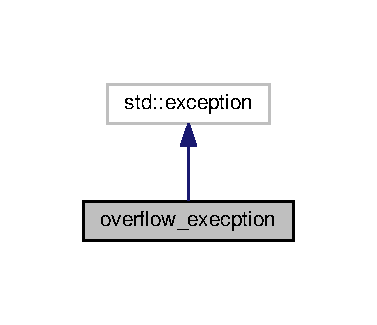
\includegraphics[width=181pt]{classoverflow__execption__inherit__graph}
\end{center}
\end{figure}


Collaboration diagram for overflow\+\_\+execption\+:\nopagebreak
\begin{figure}[H]
\begin{center}
\leavevmode
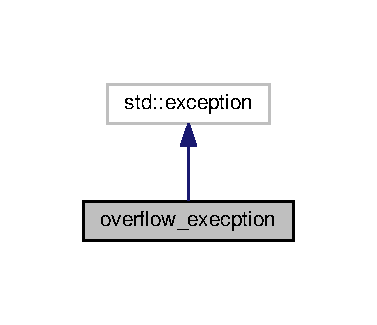
\includegraphics[width=181pt]{classoverflow__execption__coll__graph}
\end{center}
\end{figure}


\subsection{Detailed Description}
Exception invoked by integer overflow. 

This exception can be used when a number is too large. 

The documentation for this class was generated from the following file\+:\begin{DoxyCompactItemize}
\item 
\hyperlink{code__quality__professional_8cpp}{code\+\_\+quality\+\_\+professional.\+cpp}\end{DoxyCompactItemize}

\chapter{File Documentation}
\hypertarget{code__quality__professional_8cpp}{}\section{code\+\_\+quality\+\_\+professional.\+cpp File Reference}
\label{code__quality__professional_8cpp}\index{code\+\_\+quality\+\_\+professional.\+cpp@{code\+\_\+quality\+\_\+professional.\+cpp}}
{\ttfamily \#include $<$iostream$>$}\\*
{\ttfamily \#include $<$sstream$>$}\\*
{\ttfamily \#include $<$assert.\+h$>$}\\*
{\ttfamily \#include $<$exception$>$}\\*
{\ttfamily \#include $<$limits$>$}\\*
Include dependency graph for code\+\_\+quality\+\_\+professional.\+cpp\+:
\nopagebreak
\begin{figure}[H]
\begin{center}
\leavevmode
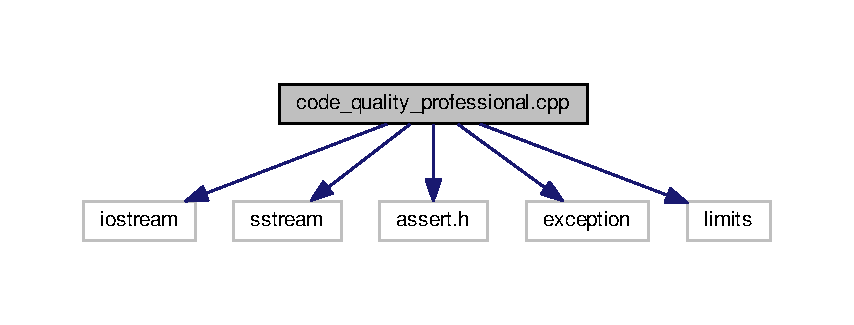
\includegraphics[width=350pt]{code__quality__professional_8cpp__incl}
\end{center}
\end{figure}
\subsection*{Classes}
\begin{DoxyCompactItemize}
\item 
class \hyperlink{classnegative__number__execption}{negative\+\_\+number\+\_\+execption}
\begin{DoxyCompactList}\small\item\em Exception invoked by negative numbers. \end{DoxyCompactList}\item 
class \hyperlink{classargument__invalid__execption}{argument\+\_\+invalid\+\_\+execption}
\begin{DoxyCompactList}\small\item\em Exception invoked by invalid arguments. \end{DoxyCompactList}\item 
class \hyperlink{classoverflow__execption}{overflow\+\_\+execption}
\begin{DoxyCompactList}\small\item\em Exception invoked by integer overflow. \end{DoxyCompactList}\end{DoxyCompactItemize}
\subsection*{Functions}
\begin{DoxyCompactItemize}
\item 
void \hyperlink{code__quality__professional_8cpp_a4c4dff898dfea5c7f94b17847e9ade8a}{argument\+To\+Integer} (char $\ast$argument, int \&number)
\begin{DoxyCompactList}\small\item\em Function converting a string to an integer. \end{DoxyCompactList}\item 
int \hyperlink{code__quality__professional_8cpp_af9f70ede9e2b2d55a963d27cbdb8346b}{calculate} (int a, int b)
\begin{DoxyCompactList}\small\item\em Calculates a!+b. \end{DoxyCompactList}\item 
int \hyperlink{code__quality__professional_8cpp_a0ddf1224851353fc92bfbff6f499fa97}{main} (int argc, char $\ast$argv\mbox{[}$\,$\mbox{]})
\begin{DoxyCompactList}\small\item\em Main function. \end{DoxyCompactList}\end{DoxyCompactItemize}


\subsection{Detailed Description}
\begin{DoxyAuthor}{Author}
Adam Leon Kleppe 
\end{DoxyAuthor}


\subsection{Function Documentation}
\hypertarget{code__quality__professional_8cpp_a4c4dff898dfea5c7f94b17847e9ade8a}{}\index{code\+\_\+quality\+\_\+professional.\+cpp@{code\+\_\+quality\+\_\+professional.\+cpp}!argument\+To\+Integer@{argument\+To\+Integer}}
\index{argument\+To\+Integer@{argument\+To\+Integer}!code\+\_\+quality\+\_\+professional.\+cpp@{code\+\_\+quality\+\_\+professional.\+cpp}}
\subsubsection[{argument\+To\+Integer}]{\setlength{\rightskip}{0pt plus 5cm}void argument\+To\+Integer (
\begin{DoxyParamCaption}
\item[{char $\ast$}]{argument, }
\item[{int \&}]{number}
\end{DoxyParamCaption}
)}\label{code__quality__professional_8cpp_a4c4dff898dfea5c7f94b17847e9ade8a}


Function converting a string to an integer. 

Converts a string opf any length to an integer if the string represents a valid integer. 
\begin{DoxyExceptions}{Exceptions}
{\em \hyperlink{classargument__invalid__execption}{argument\+\_\+invalid\+\_\+execption}} & if the argument is not a valid integer. \\
\hline
\end{DoxyExceptions}

\begin{DoxyParams}{Parameters}
{\em argument} & The argument which is supposed to converted. \\
\hline
{\em number} & The output number of the conversion \\
\hline
\end{DoxyParams}
\hypertarget{code__quality__professional_8cpp_af9f70ede9e2b2d55a963d27cbdb8346b}{}\index{code\+\_\+quality\+\_\+professional.\+cpp@{code\+\_\+quality\+\_\+professional.\+cpp}!calculate@{calculate}}
\index{calculate@{calculate}!code\+\_\+quality\+\_\+professional.\+cpp@{code\+\_\+quality\+\_\+professional.\+cpp}}
\subsubsection[{calculate}]{\setlength{\rightskip}{0pt plus 5cm}int calculate (
\begin{DoxyParamCaption}
\item[{int}]{a, }
\item[{int}]{b}
\end{DoxyParamCaption}
)}\label{code__quality__professional_8cpp_af9f70ede9e2b2d55a963d27cbdb8346b}


Calculates a!+b. 

Calculates the equation a! + b 
\begin{DoxyExceptions}{Exceptions}
{\em \hyperlink{classnegative__number__execption}{negative\+\_\+number\+\_\+execption}} & if a is negative \\
\hline
{\em \hyperlink{classoverflow__execption}{overflow\+\_\+execption}} & if either a or the result is larger than I\+N\+T\+\_\+\+M\+A\+X \\
\hline
\end{DoxyExceptions}

\begin{DoxyParams}{Parameters}
{\em a} & Integer which will be factorialized \\
\hline
{\em b} & Integer which will be added \\
\hline
\end{DoxyParams}
\begin{DoxyReturn}{Returns}
The result of the equation a!+b 
\end{DoxyReturn}
\hypertarget{code__quality__professional_8cpp_a0ddf1224851353fc92bfbff6f499fa97}{}\index{code\+\_\+quality\+\_\+professional.\+cpp@{code\+\_\+quality\+\_\+professional.\+cpp}!main@{main}}
\index{main@{main}!code\+\_\+quality\+\_\+professional.\+cpp@{code\+\_\+quality\+\_\+professional.\+cpp}}
\subsubsection[{main}]{\setlength{\rightskip}{0pt plus 5cm}int main (
\begin{DoxyParamCaption}
\item[{int}]{argc, }
\item[{char $\ast$}]{argv\mbox{[}$\,$\mbox{]}}
\end{DoxyParamCaption}
)}\label{code__quality__professional_8cpp_a0ddf1224851353fc92bfbff6f499fa97}


Main function. 

Takes in two arguments which are numbers a and b, and outputs the result of the equation a! + b. 
\begin{DoxyParams}{Parameters}
{\em argc} & The number of arguments \\
\hline
{\em argv} & Array containing all the arguments. \\
\hline
\end{DoxyParams}
\begin{DoxyReturn}{Returns}
0 if the computation was successful, and -\/1 if it failed. 
\end{DoxyReturn}

%--- End generated contents ---

% Index
\backmatter
\newpage
\phantomsection
\clearemptydoublepage
\addcontentsline{toc}{chapter}{Index}
\printindex

\end{document}
